\chapter{Prolog}


It may be useful to first have a look at the "Logic programming" section of 
\href{https://github.com/NotXia/unibo-ai-notes/tree/pdfs/languages-and-algorithms-for-ai/module2}{\texttt{Languages and Algorithms for AI (module 2)}}.


\section{Syntax}

\begin{description}
    \item[Term] \marginnote{Term}
        Following the first-order logic definition, a term can be a:
        \begin{itemize}
            \item Constant (\texttt{lowerCase}).
            \item Variable (\texttt{UpperCase}).
            \item Function symbol (\texttt{f(t1, \dots, tn)} with \texttt{t1}, \dots, \texttt{tn} terms).
        \end{itemize}

    \item[Atomic formula] \marginnote{Atomic formula}
        An atomic formula has form:
        \[ \texttt{p(t1, \dots, tn)} \]
        where \texttt{p} is a predicate symbol and \texttt{t1}, \dots, \texttt{tn} are terms.

        Note: there are no syntactic distinctions between constants, functions and predicates.

    \item[Clause] \marginnote{Horn clause}
        A Prolog program is a set of horn clauses:
        \begin{descriptionlist}
            \item[Fact] \texttt{A.}
            \item[Rule] \texttt{A :- B1, \dots, Bn.} (\texttt{A} is the head and \texttt{B1, \dots, Bn} the body)
            \item[Goal] \texttt{:- B1, \dots, Bn.}
        \end{descriptionlist}
        where:
        \begin{itemize}
            \item \texttt{A}, \texttt{B1}, \dots, \texttt{Bn} are atomic formulas.
            \item \texttt{,} represents the conjunction ($\land$).
            \item \texttt{:-} represents the logical implication ($\Leftarrow$).
        \end{itemize}

        \begin{description}
            \item[Quantification] \marginnote{Quantification} \phantom{}
                \begin{description}
                    \item[Facts] 
                        Variables appearing in a fact are quantified universally.
                        \[ \texttt{A(X).} \equiv \forall \texttt{X}: \texttt{A(X)}  \]
                    \item[Rules] 
                        Variables appearing the the body only are quantified existentially.
                        Variables appearing in both the head and the body are quantified universally.
                        \[ \texttt{A(X) :- B(X, Y).} \equiv \forall \texttt{X}, \exists \texttt{Y} : \texttt{A(X)} \Leftarrow \texttt{B(X, Y)} \]

                    \item[Goals] 
                        Variables are quantified existentially.
                        \[ \texttt{:- B(Y).} \equiv \exists \texttt{Y} : \texttt{B(Y)}  \]
                \end{description}
        \end{description}
\end{description}


\section{Semantics}

\begin{description}
    \item[Execution of a program]
        A computation in Prolog attempts to prove the goal.
        Given a program $P$ and a goal \texttt{:- p(t1, \dots, tn)},
        the objective is to find a substitution $\sigma$ such that:
        \[ P \models [\, \texttt{p(t1, \dots, tn)} \,]\sigma \]

        In practice, it uses two stacks:
        \begin{descriptionlist}
            \item[Execution stack] Contains the predicates the interpreter is trying to prove.
            \item[Backtracking stack] Contains the choice points (clauses) the interpreter can try.
        \end{descriptionlist}

    \item[SLD resolution] \marginnote{SLD}
        Prolog uses SLD resolution with the following choices:
        \begin{descriptionlist}
            \item[Left-most] Always proves the left-most literal first.
            \item[Depth-first] Applies the predicates following the order of definition.
        \end{descriptionlist}

        Note that the depth-first approach can be efficiently implemented (tail recursion)
        but the termination of a Prolog program on a provable goal is not guaranteed as it may loop depending on the ordering of the clauses.

    \item[Disjunction operator]
        The operator \texttt{;} can be seen as a disjunction and makes the Prolog interpreter
        explore the remaining SLD tree looking for alternative solutions.
\end{description}



\section{Arithmetic operators}
\marginnote{Arithmetic operators}

In Prolog:
\begin{itemize}
    \item Integers and floating points are built-in atoms.
    \item Math operators are built-in function symbols.
\end{itemize}
Therefore, mathematical expressions are terms.

\begin{description}
    \item[\texttt{is} predicate]
        The predicate \texttt{is} is used to evaluate and unify expressions:
        \[ \texttt{T is Expr} \]
        where \texttt{T} is a numerical atom or a variable and \texttt{Expr} is an expression without free variables.
        After evaluation, the result of \texttt{Expr} is unified with \texttt{T}.

        \begin{example} \phantom{}
            \begin{lstlisting}[language={}]
    :- X is 2+3.
    yes X=5
            \end{lstlisting}
        \end{example}

        Note: a term representing an expression is evaluated only with the predicate \texttt{is} (otherwise it remains as is).

    \item[Relational operators]
        Relational operators (\texttt{>}, \texttt{<}, \texttt{>=}, \texttt{=<}, \texttt{==}, \texttt{=/=}) are built-in.
\end{description}



\section{Lists}
\marginnote{Lists}

A list is defined recursively as:
\begin{descriptionlist}
    \item[Empty list] \texttt{[]}
    \item[List constructor] \texttt{.(T, L)} where \texttt{T} is a term and \texttt{L} is a list.
\end{descriptionlist}
Note that a list always ends with an empty list.

As the formal definition is impractical, some syntactic sugar has been defined:
\begin{descriptionlist}
    \item[List definition] \texttt{[t1, \dots, tn]} can be used to define a list.  
    \item[Head and tail] \texttt{[H | T]} where \texttt{H} is the head (term) and \texttt{T} the tail (list) can be useful for recursive calls.
\end{descriptionlist}



\section{Cut}
\marginnote{Cut}

The cut operator (\texttt{!}) allows to control the exploration of the SLD tree.

A cut in a clause:
\[ \texttt{p :- q1, \dots, qi, !, qj, \dots, qn.} \]
makes the interpreter consider only the first choice points for \texttt{q1, \dots, qi}, dropping all the other possibilities.
Therefore, if \texttt{qj, \dots, qn} fails, there won't be backtracking and \texttt{p} fails.

\begin{example} \phantom{}\\[0.5em]
    \begin{minipage}{0.5\textwidth}
        \begin{lstlisting}
    p(X) :- q(X), r(X).
    q(1).
    q(2).
    r(2).

    :- p(X).
    yes X=2
        \end{lstlisting}
    \end{minipage}
    \begin{minipage}{0.5\textwidth}
        \begin{lstlisting}
    p(X) :- q(X), !, r(X).
    q(1).
    q(2).
    r(2).

    :- p(X).
    no
        \end{lstlisting}
    \end{minipage}

    In the second case, the cut drops the choice point \texttt{q(2)} and only considers \texttt{q(1)}.
\end{example}

\begin{description}
    \item[Mutual exclusion]
        A cut can be useful to achieve mutual exclusion.
        In other words, to represent a conditional branching:
        \[ \texttt{if a(X) then b else c} \]
        a cut can be used as follows:
        \begin{lstlisting}
    p(X) :- a(X), !, b.
    p(X) :- c.
        \end{lstlisting}

        If \texttt{a(X)} succeeds, other choice points for \texttt{p} will be dropped and only \texttt{b} will be evaluated.
        If \texttt{a(X)} fails, the second clause will be considered, therefore evaluating \texttt{c}.
\end{description}



\section{Negation}

\begin{description}
    \item[Closed-world assumption] \marginnote{Closed-world assumption}
        Only what is stated in a program $P$ is true, everything else is false:
        \[ \texttt{CWA}(P) = P \cup \{ \lnot A \mid A \text{ is a ground atomic formula and } P \cancel{\models} A \} \]

        \begin{description}
            \item[Non-monotonic inference rule]
                Adding new axioms to the program may change the set of valid theorems. 
        \end{description}

        As first-order logic in undecidable, closed-world assumption cannot be directly applied in practice.

    \item[Negation as failure] \marginnote{Negation as failure}
        A negated atom $\lnot A$ is considered true iff $A$ fails in finite time:
        \[ \texttt{NF}(P) = P \cup \{ \lnot A \mid A \in \texttt{FF}(P) \} \]
        where $\texttt{FF}(P) = \{ B \mid P \cancel{\models} B \text{ in finite time} \}$ 
        is the set of atoms for which the proof fails in finite time.
        Note that not all atoms $B$ such that $P \cancel{\models} B$ are in $\texttt{FF}(P)$.

    \item[SLDNF] \marginnote{SLDNF}
        SLD resolution with NF to solve negative atoms.
        
        Given a goal of literals \texttt{:- L$_1$, \dots, L$_m$}, SLDNF does the following:
        \begin{enumerate}
            \item Select a positive or ground negative literal \texttt{L$_i$}:
                \begin{itemize}
                    \item If \texttt{L$_i$} is positive, apply the normal SLD resolution.
                    \item If \texttt{L$_i$} = $\lnot A$, prove that $A$ fails in finite time. 
                        If it succeeds, \texttt{L$_i$} fails.
                \end{itemize}
            \item Solve the goal \texttt{:- L$_1$, \dots, L$_{i-1}$, L$_{i+1}$, \dots  L$_m$}.
        \end{enumerate}

        \begin{theorem}
            If only positive or ground negative literal are selected during resolution, SLDNF is correct and complete.
        \end{theorem}

        \begin{description}
            \item[Prolog SLDNF] 
                Prolog uses an incorrect implementation of SLDNF where the selection rule always chooses the left-most literal.
                This potentially causes incorrect deductions.

                \begin{proof}
                    When proving \texttt{:- \char`\\+capital(X).}, the intended meaning is:
                    \[ \exists \texttt{X}: \lnot \texttt{capital(X)}  \]

                    In SLDNF, to prove \texttt{:- \char`\\+capital(X).}, the algorithm proves \texttt{:- capital(X).}, which results in:
                    \[ \exists \texttt{X}: \texttt{capital(X)}  \]
                    and then negates the result, which corresponds to:
                    \[ \lnot (\exists \texttt{X}: \texttt{capital(X)}) \iff \forall \texttt{X}: (\lnot \texttt{capital(X)}) \]

                \end{proof}

                \begin{example}[Correct SLDNF resolution]
                    Given the program:
                    \begin{lstlisting}[language={}, mathescape=true]
    capital(rome).
    region_capital(bologna).
    city(X) :- capital(X).
    city(X) :- region_capital(X).

    :- city(X), \+capital(X).
                    \end{lstlisting}
                    its resolution succeeds with \texttt{X=bologna} as \texttt{\char`\\+capital(X)} is ground by the unification of \texttt{city(X)}.
                    \begin{center}
                        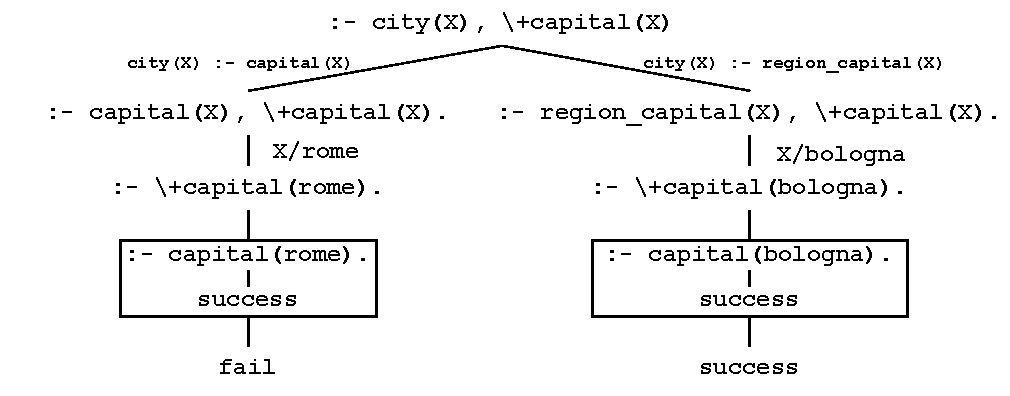
\includegraphics[width=0.75\textwidth]{img/_sldnf_correct_example.pdf}
                    \end{center}
                \end{example}

                \begin{example}[Incorrect SLDNF resolution] 
                    Given the program: \\
                    \begin{minipage}{0.45\textwidth}
                        \begin{lstlisting}[language={}, mathescape=true]
    capital(rome).
    region_capital(bologna).
    city(X) :- capital(X).
    city(X) :- region_capital(X).

    :- \+capital(X), city(X).
                        \end{lstlisting}
                    \end{minipage}
                    \begin{minipage}{0.5\textwidth}
                        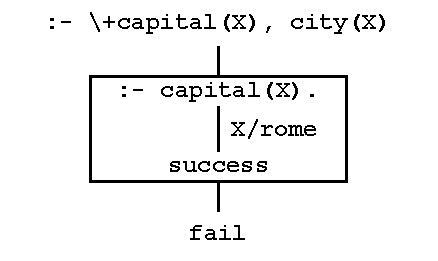
\includegraphics[width=0.7\linewidth]{img/_sldnf_incorrect_example.pdf}
                    \end{minipage}

                    its resolution fails as \texttt{\char`\\+capital(X)} is a free variable and 
                    the proof of \texttt{capital(X)} is ground with \texttt{X=rome} and succeeds, therefore failing \texttt{\char`\\+capital(X)}.
                    Note that \texttt{bologna} is not tried as it does not appear in the axioms of \texttt{capital}.
                \end{example}
        \end{description}
\end{description}